% Generated from example/sample.drawio page 1 via drawio SVG.
% The intermediate SVG was sanitized by drawio2tikz.
\definecolor{cababab}{RGB}{171,171,171}
\definecolor{cd4d4d4}{RGB}{212,212,212}
\definecolor{cff8000}{RGB}{255,128,0}

\def \globalscale {1.000000}
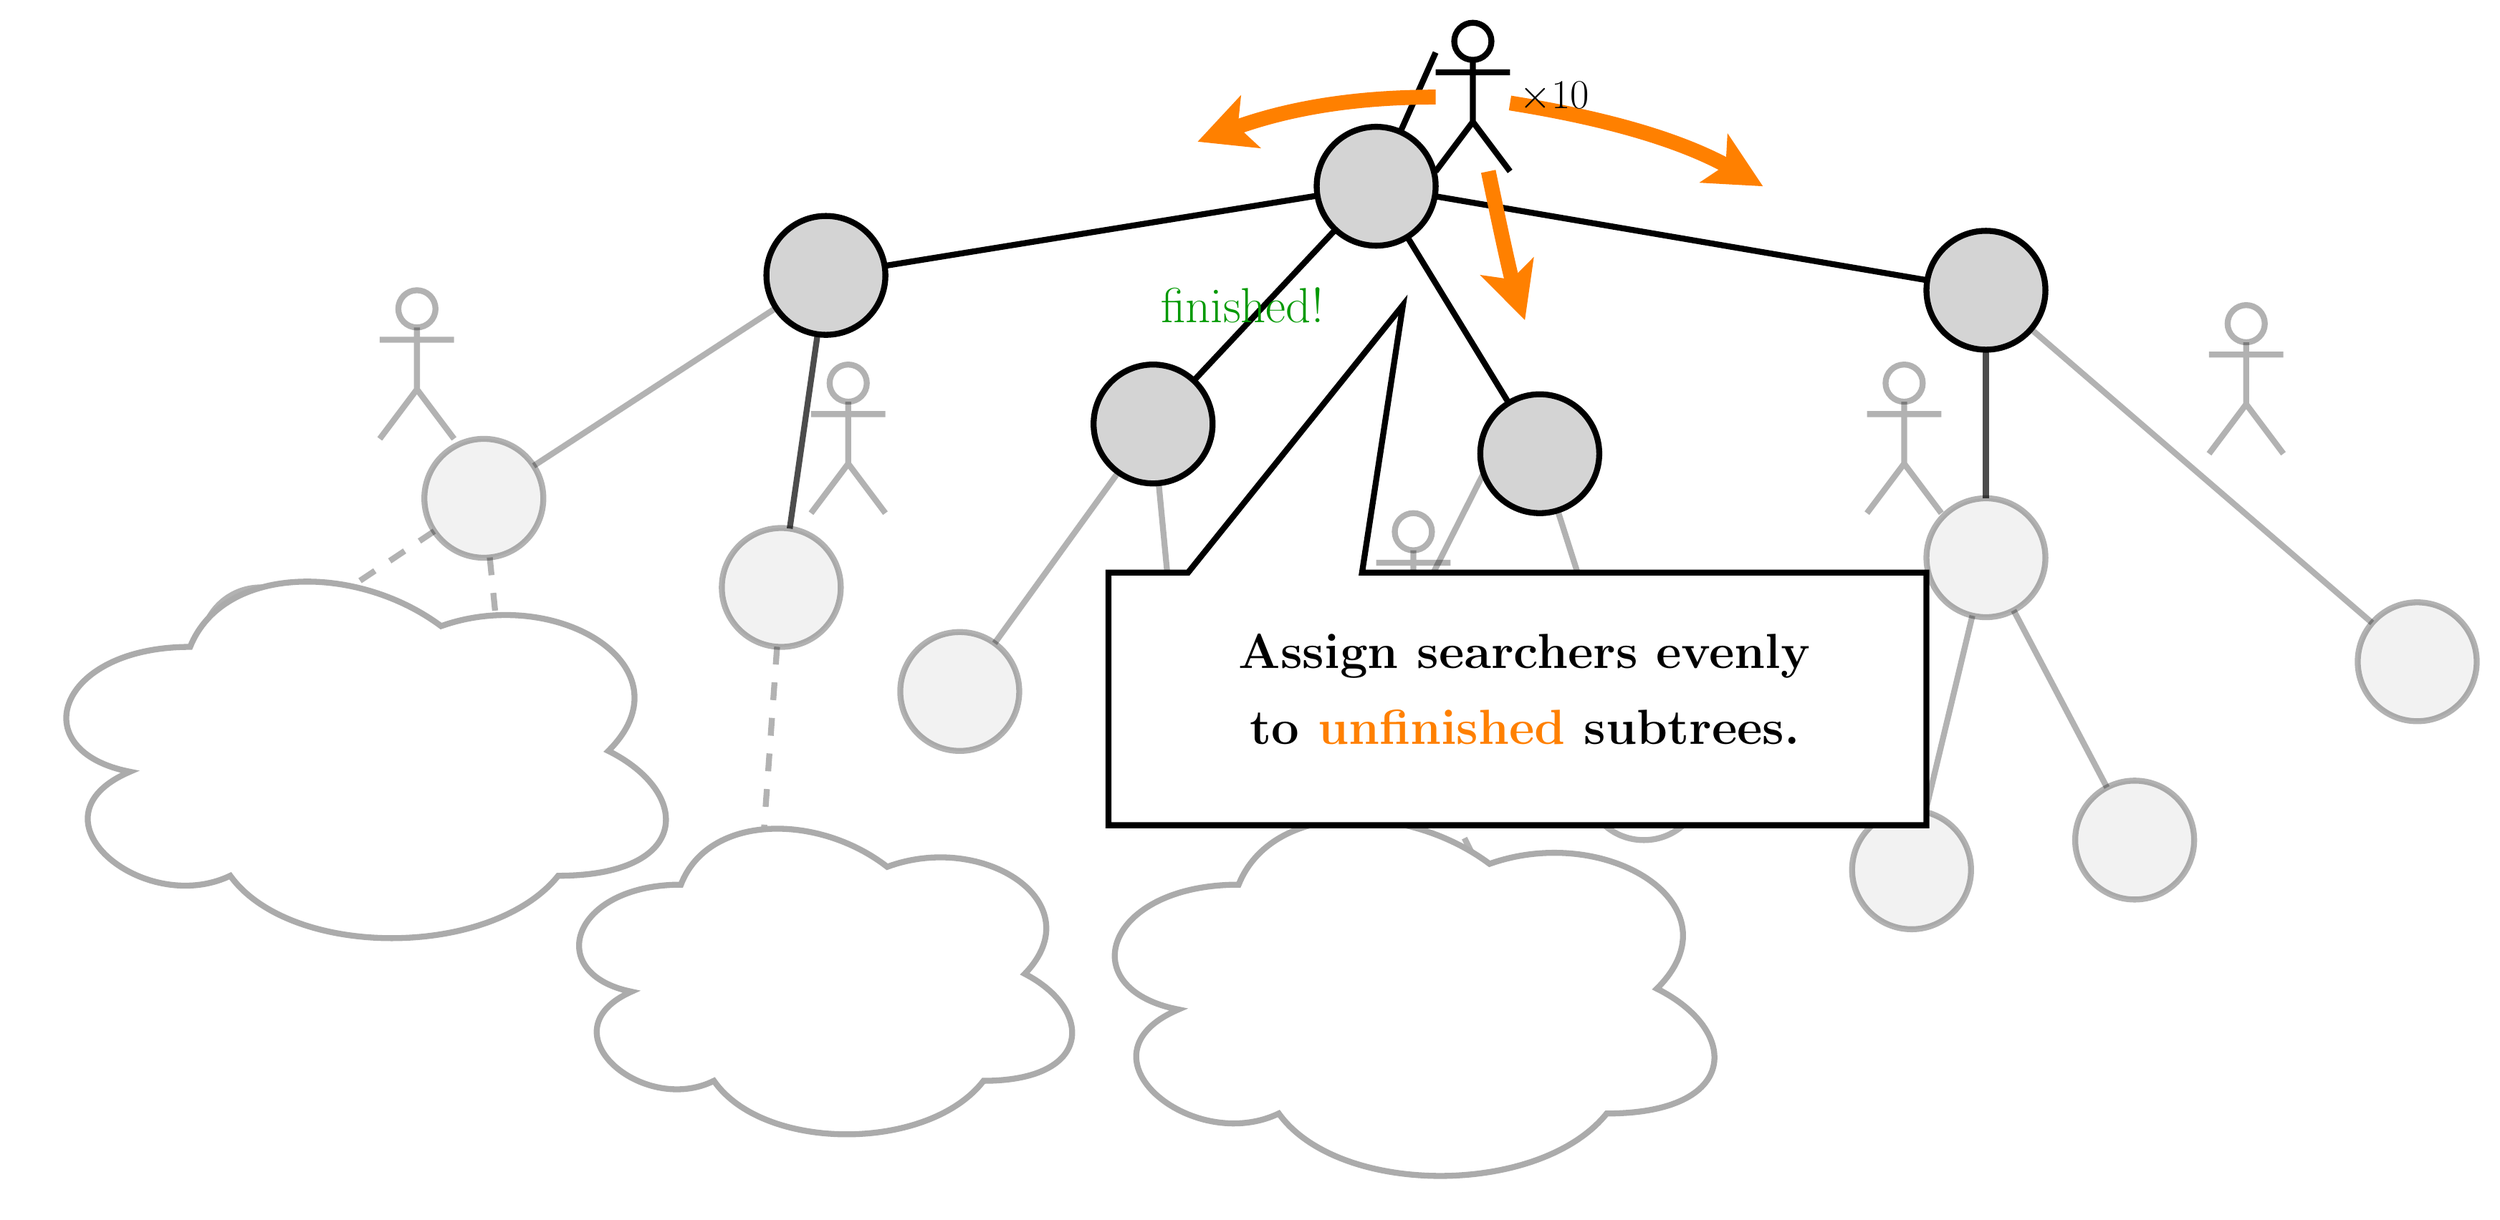
\begin{tikzpicture}[y=1pt, x=1pt, yscale=\globalscale, xscale=\globalscale, every node/.append style={scale=\globalscale}, inner sep=0pt, outer sep=0pt]
  \path[draw=black,line width=3pt,miter limit=10] (654.382, 506.745) -- (436.11, 471.3);

  \path[draw=black,line width=3pt,miter limit=10] (663.472, 489.623) -- (592.02, 413.385);

  \path[draw=black,line width=3pt,miter limit=10] (699.69, 485.933) -- (750.855, 402.097);

  \path[draw=black,line width=3pt,miter limit=10] (713.572, 506.467) -- (961.928, 464.048);

  \path[draw=black,line width=3pt,miter limit=10] (696.188, 538.912) -- (714, 579);

  \path[draw=black,line width=3pt,miter limit=4,fill=cd4d4d4] (714, 511.5) .. controls (714, 494.931) and (700.569, 481.5) .. (684, 481.5) .. controls (667.431, 481.5) and (654, 494.931) .. (654, 511.5) .. controls (654, 528.069) and (667.431, 541.5) .. (684, 541.5) .. controls (700.569, 541.5) and (714, 528.069) .. (714, 511.5) -- cycle;

  \path[draw=black,line width=3pt,draw opacity=0.3,miter limit=10] (381.382, 450.097) -- (259.125, 370.388);

  \path[draw=black,line width=3pt,draw opacity=0.7,miter limit=10] (402.308, 436.793) -- (388.245, 338.7);

  \path[draw=black,line width=3pt,miter limit=4,fill=cd4d4d4] (436.5, 466.5) .. controls (436.5, 449.931) and (423.069, 436.5) .. (406.5, 436.5) .. controls (389.931, 436.5) and (376.5, 449.931) .. (376.5, 466.5) .. controls (376.5, 483.069) and (389.931, 496.5) .. (406.5, 496.5) .. controls (423.069, 496.5) and (436.5, 483.069) .. (436.5, 466.5) -- cycle;

  \path[draw=black,line width=3pt,draw opacity=0.3,miter limit=10] (553.95, 367.17) -- (491.565, 280.822);

  \path[draw=black,line width=3pt,draw opacity=0.3,miter limit=10] (574.312, 361.635) -- (583.658, 263.865);

  \path[draw=black,line width=3pt,miter limit=4,fill=cd4d4d4] (601.5, 391.5) .. controls (601.5, 374.931) and (588.069, 361.5) .. (571.5, 361.5) .. controls (554.931, 361.5) and (541.5, 374.931) .. (541.5, 391.5) .. controls (541.5, 408.069) and (554.931, 421.5) .. (571.5, 421.5) .. controls (588.069, 421.5) and (601.5, 408.069) .. (601.5, 391.5) -- cycle;

  \path[draw=black,line width=3pt,draw opacity=0.3,miter limit=10] (775.507, 347.888) -- (809.902, 240.09);

  \path[draw=black,line width=3pt,draw opacity=0.3,miter limit=10] (738.217, 366.795) -- (697.305, 285.585);

  \path[draw=black,line width=3pt,miter limit=4,fill=cd4d4d4] (796.5, 376.5) .. controls (796.5, 359.931) and (783.069, 346.5) .. (766.5, 346.5) .. controls (749.931, 346.5) and (736.5, 359.931) .. (736.5, 376.5) .. controls (736.5, 393.069) and (749.931, 406.5) .. (766.5, 406.5) .. controls (783.069, 406.5) and (796.5, 393.069) .. (796.5, 376.5) -- cycle;

  \path[draw=black,line width=3pt,draw opacity=0.3,miter limit=10] (1014.232, 439.425) -- (1186.275, 291.09);

  \path[draw=black,line width=3pt,draw opacity=0.7,miter limit=10] (991.5, 429) -- (991.5, 354);

  \path[draw=black,line width=3pt,miter limit=4,fill=cd4d4d4] (1021.5, 459) .. controls (1021.5, 442.431) and (1008.069, 429) .. (991.5, 429) .. controls (974.931, 429) and (961.5, 442.431) .. (961.5, 459) .. controls (961.5, 475.569) and (974.931, 489) .. (991.5, 489) .. controls (1008.069, 489) and (1021.5, 475.569) .. (1021.5, 459) -- cycle;

  \path[draw=black,line width=3pt,draw opacity=0.3,miter limit=10,dash pattern=on 9pt off 9pt] (209.002, 337.41) -- (146.46, 295.642);

  \path[draw=black,line width=3pt,draw opacity=0.3,miter limit=10,dash pattern=on 9pt off 9pt] (236.985, 324.15) -- (246.015, 233.85);

  \path[draw=black,line width=3pt,draw opacity=0.3,miter limit=4,fill=cd4d4d4,fill opacity=0.3] (264, 354) .. controls (264, 337.431) and (250.569, 324) .. (234, 324) .. controls (217.431, 324) and (204, 337.431) .. (204, 354) .. controls (204, 370.569) and (217.431, 384) .. (234, 384) .. controls (250.569, 384) and (264, 370.569) .. (264, 354) -- cycle;

  \path[draw=black,line width=3pt,draw opacity=0.3,miter limit=4,fill=white,fill opacity=0.3] (399, 99) .. controls (399, 82.431) and (385.569, 69) .. (369, 69) .. controls (352.431, 69) and (339, 82.431) .. (339, 99) .. controls (339, 115.569) and (352.431, 129) .. (369, 129) .. controls (385.569, 129) and (399, 115.569) .. (399, 99) -- cycle;

  \path[draw=black,line width=3pt,draw opacity=0.3,miter limit=10,dash pattern=on 9pt off 9pt] (381.877, 279.075) -- (371.138, 128.925);

  \path[draw=black,line width=3pt,draw opacity=0.3,miter limit=4,fill=cd4d4d4,fill opacity=0.3] (414, 309) .. controls (414, 292.431) and (400.569, 279) .. (384, 279) .. controls (367.431, 279) and (354, 292.431) .. (354, 309) .. controls (354, 325.569) and (367.431, 339) .. (384, 339) .. controls (400.569, 339) and (414, 325.569) .. (414, 309) -- cycle;

  \path[draw=black,line width=3pt,draw opacity=0.3,miter limit=4,fill=cd4d4d4,fill opacity=0.3] (504, 256.5) .. controls (504, 239.931) and (490.569, 226.5) .. (474, 226.5) .. controls (457.431, 226.5) and (444, 239.931) .. (444, 256.5) .. controls (444, 273.069) and (457.431, 286.5) .. (474, 286.5) .. controls (490.569, 286.5) and (504, 273.069) .. (504, 256.5) -- cycle;

  \path[draw=black,line width=3pt,draw opacity=0.3,miter limit=4,fill=white,fill opacity=0.3] (616.5, 234) .. controls (616.5, 217.431) and (603.069, 204) .. (586.5, 204) .. controls (569.931, 204) and (556.5, 217.431) .. (556.5, 234) .. controls (556.5, 250.569) and (569.931, 264) .. (586.5, 264) .. controls (603.069, 264) and (616.5, 250.569) .. (616.5, 234) -- cycle;

  \path[draw=black,line width=3pt,draw opacity=0.3,miter limit=4,fill=white,fill opacity=0.3] (849, 211.5) .. controls (849, 194.931) and (835.569, 181.5) .. (819, 181.5) .. controls (802.431, 181.5) and (789, 194.931) .. (789, 211.5) .. controls (789, 228.069) and (802.431, 241.5) .. (819, 241.5) .. controls (835.569, 241.5) and (849, 228.069) .. (849, 211.5) -- cycle;

  \path[draw=black,line width=3pt,draw opacity=0.3,miter limit=10] (690.428, 212.752) -- (662.618, 120.232);

  \path[draw=black,line width=3pt,draw opacity=0.3,miter limit=10,dash pattern=on 9pt off 9pt] (712.418, 214.665) -- (753.082, 133.335);

  \path[draw=black,line width=3pt,draw opacity=0.3,miter limit=4,fill=white,fill opacity=0.3] (729, 241.5) .. controls (729, 224.931) and (715.569, 211.5) .. (699, 211.5) .. controls (682.431, 211.5) and (669, 224.931) .. (669, 241.5) .. controls (669, 258.069) and (682.431, 271.5) .. (699, 271.5) .. controls (715.569, 271.5) and (729, 258.069) .. (729, 241.5) -- cycle;

  \path[draw=black,line width=3pt,draw opacity=0.3,miter limit=4,fill=white,fill opacity=0.3] (684, 91.5) .. controls (684, 74.931) and (670.569, 61.5) .. (654, 61.5) .. controls (637.431, 61.5) and (624, 74.931) .. (624, 91.5) .. controls (624, 108.069) and (637.431, 121.5) .. (654, 121.5) .. controls (670.569, 121.5) and (684, 108.069) .. (684, 91.5) -- cycle;

  \path[draw=black,line width=3pt,draw opacity=0.3,miter limit=4,fill=white,fill opacity=0.3] (796.5, 106.5) .. controls (796.5, 89.931) and (783.069, 76.5) .. (766.5, 76.5) .. controls (749.931, 76.5) and (736.5, 89.931) .. (736.5, 106.5) .. controls (736.5, 123.069) and (749.931, 136.5) .. (766.5, 136.5) .. controls (783.069, 136.5) and (796.5, 123.069) .. (796.5, 106.5) -- cycle;

  \path[draw=black,line width=3pt,draw opacity=0.3,miter limit=4,fill=cd4d4d4,fill opacity=0.3] (1239, 271.5) .. controls (1239, 254.931) and (1225.569, 241.5) .. (1209, 241.5) .. controls (1192.431, 241.5) and (1179, 254.931) .. (1179, 271.5) .. controls (1179, 288.069) and (1192.431, 301.5) .. (1209, 301.5) .. controls (1225.569, 301.5) and (1239, 288.069) .. (1239, 271.5) -- cycle;

  \path[draw=black,line width=3pt,draw opacity=0.3,miter limit=10] (1005.465, 297.45) -- (1052.527, 208.05);

  \path[draw=black,line width=3pt,draw opacity=0.3,miter limit=10] (984.668, 294.788) -- (960.945, 195.682);

  \path[draw=black,line width=3pt,draw opacity=0.3,miter limit=4,fill=cd4d4d4,fill opacity=0.3] (1021.5, 324) .. controls (1021.5, 307.431) and (1008.069, 294) .. (991.5, 294) .. controls (974.931, 294) and (961.5, 307.431) .. (961.5, 324) .. controls (961.5, 340.569) and (974.931, 354) .. (991.5, 354) .. controls (1008.069, 354) and (1021.5, 340.569) .. (1021.5, 324) -- cycle;

  \path[draw=black,line width=3pt,draw opacity=0.3,miter limit=4,fill=cd4d4d4,fill opacity=0.3] (1096.5, 181.5) .. controls (1096.5, 164.931) and (1083.069, 151.5) .. (1066.5, 151.5) .. controls (1049.931, 151.5) and (1036.5, 164.931) .. (1036.5, 181.5) .. controls (1036.5, 198.069) and (1049.931, 211.5) .. (1066.5, 211.5) .. controls (1083.069, 211.5) and (1096.5, 198.069) .. (1096.5, 181.5) -- cycle;

  \path[draw=black,line width=3pt,draw opacity=0.3,miter limit=4,fill=cd4d4d4,fill opacity=0.3] (984, 166.5) .. controls (984, 149.931) and (970.569, 136.5) .. (954, 136.5) .. controls (937.431, 136.5) and (924, 149.931) .. (924, 166.5) .. controls (924, 183.069) and (937.431, 196.5) .. (954, 196.5) .. controls (970.569, 196.5) and (984, 183.069) .. (984, 166.5) -- cycle;

  \path[draw=black,line width=3pt,draw opacity=0.3,miter limit=4,fill=white,fill opacity=0.3] (279, 204) .. controls (279, 187.431) and (265.569, 174) .. (249, 174) .. controls (232.431, 174) and (219, 187.431) .. (219, 204) .. controls (219, 220.569) and (232.431, 234) .. (249, 234) .. controls (265.569, 234) and (279, 220.569) .. (279, 204) -- cycle;

  \path[draw=black,line width=3pt,draw opacity=0.3,miter limit=4,fill=white,fill opacity=0.3] (151.5, 279) .. controls (151.5, 262.431) and (138.069, 249) .. (121.5, 249) .. controls (104.931, 249) and (91.5, 262.431) .. (91.5, 279) .. controls (91.5, 295.569) and (104.931, 309) .. (121.5, 309) .. controls (138.069, 309) and (151.5, 295.569) .. (151.5, 279) -- cycle;

  \path[draw=cababab,line width=3pt,miter limit=10,fill=white] (614.625, 159) .. controls (547.125, 159) and (530.25, 106.5) .. (584.25, 96) .. controls (530.25, 72.9) and (591, 22.5) .. (634.875, 43.5) .. controls (665.25, 1.5) and (766.5, 1.5) .. (800.25, 43.5) .. controls (867.75, 43.5) and (867.75, 85.5) .. (825.562, 106.5) .. controls (867.75, 148.5) and (800.25, 190.5) .. (741.188, 169.5) .. controls (699, 201) and (631.5, 201) .. (614.625, 159) -- cycle;

  \path[draw=cababab,line width=3pt,miter limit=10,fill=white] (333.375, 159) .. controls (277.875, 159) and (264, 114) .. (308.4, 105) .. controls (264, 85.2) and (313.95, 42) .. (350.025, 60) .. controls (375, 24) and (458.25, 24) .. (486, 60) .. controls (541.5, 60) and (541.5, 96) .. (506.812, 114) .. controls (541.5, 150) and (486, 186) .. (437.438, 168) .. controls (402.75, 195) and (347.25, 195) .. (333.375, 159) -- cycle;

  \path[draw=cababab,line width=3pt,miter limit=10,fill=white] (85.875, 279) .. controls (18.375, 279) and (1.5, 226.5) .. (55.5, 216) .. controls (1.5, 192.9) and (62.25, 142.5) .. (106.125, 163.5) .. controls (136.5, 121.5) and (237.75, 121.5) .. (271.5, 163.5) .. controls (339, 163.5) and (339, 205.5) .. (296.812, 226.5) .. controls (339, 268.5) and (271.5, 310.5) .. (212.438, 289.5) .. controls (170.25, 321) and (102.75, 321) .. (85.875, 279) -- cycle;

  \path[draw=black,line width=3pt,draw opacity=0.3,miter limit=4,fill=white,fill opacity=0.3] (209.625, 449.625) .. controls (209.625, 444.447) and (205.428, 440.25) .. (200.25, 440.25) .. controls (195.072, 440.25) and (190.875, 444.447) .. (190.875, 449.625) .. controls (190.875, 454.803) and (195.072, 459) .. (200.25, 459) .. controls (205.428, 459) and (209.625, 454.803) .. (209.625, 449.625) -- cycle;

  \path[draw=black,line width=3pt,draw opacity=0.3,miter limit=10] (200.25, 440.25) -- (200.25, 408.998) (200.25, 434.002) -- (181.5, 434.002) (200.25, 434.002) -- (219, 434.002) (200.25, 408.998) -- (181.5, 384) (200.25, 408.998) -- (219, 384);

  \path[draw=black,line width=3pt,draw opacity=0.3,miter limit=4,fill=white,fill opacity=0.3] (427.125, 412.125) .. controls (427.125, 406.947) and (422.928, 402.75) .. (417.75, 402.75) .. controls (412.572, 402.75) and (408.375, 406.947) .. (408.375, 412.125) .. controls (408.375, 417.303) and (412.572, 421.5) .. (417.75, 421.5) .. controls (422.928, 421.5) and (427.125, 417.303) .. (427.125, 412.125) -- cycle;

  \path[draw=black,line width=3pt,draw opacity=0.3,miter limit=10] (417.75, 402.75) -- (417.75, 371.498) (417.75, 396.503) -- (399, 396.503) (417.75, 396.503) -- (436.5, 396.503) (417.75, 371.498) -- (399, 346.5) (417.75, 371.498) -- (436.5, 346.5);

  \path[draw=black,line width=3pt,draw opacity=0.3,miter limit=4,fill=white,fill opacity=0.3] (712.125, 337.125) .. controls (712.125, 331.947) and (707.928, 327.75) .. (702.75, 327.75) .. controls (697.572, 327.75) and (693.375, 331.947) .. (693.375, 337.125) .. controls (693.375, 342.303) and (697.572, 346.5) .. (702.75, 346.5) .. controls (707.928, 346.5) and (712.125, 342.303) .. (712.125, 337.125) -- cycle;

  \path[draw=black,line width=3pt,draw opacity=0.3,miter limit=10] (702.75, 327.75) -- (702.75, 296.498) (702.75, 321.502) -- (684, 321.502) (702.75, 321.502) -- (721.5, 321.502) (702.75, 296.498) -- (684, 271.5) (702.75, 296.498) -- (721.5, 271.5);

  \path[draw=black,line width=3pt,draw opacity=0.3,miter limit=4,fill=white,fill opacity=0.3] (959.625, 412.125) .. controls (959.625, 406.947) and (955.428, 402.75) .. (950.25, 402.75) .. controls (945.072, 402.75) and (940.875, 406.947) .. (940.875, 412.125) .. controls (940.875, 417.303) and (945.072, 421.5) .. (950.25, 421.5) .. controls (955.428, 421.5) and (959.625, 417.303) .. (959.625, 412.125) -- cycle;

  \path[draw=black,line width=3pt,draw opacity=0.3,miter limit=10] (950.25, 402.75) -- (950.25, 371.498) (950.25, 396.503) -- (931.5, 396.503) (950.25, 396.503) -- (969, 396.503) (950.25, 371.498) -- (931.5, 346.5) (950.25, 371.498) -- (969, 346.5);

  \path[draw=cff8000,line width=7.5pt,miter limit=10] (740.565, 519) .. controls (747.855, 484) and (752.168, 464.498) .. (753.502, 460.493);

  \path[draw=cff8000,line width=7.5pt,miter limit=10,fill=cff8000] (756.345, 451.957) -- (746.865, 461.445) -- (753.502, 460.493) -- (758.243, 465.24) -- cycle;

  \path[draw=cff8000,line width=7.5pt,miter limit=10] (751.5, 553.5) .. controls (801.5, 545.5) and (838.967, 534.375) .. (863.902, 520.125);

  \path[draw=cff8000,line width=7.5pt,miter limit=10,fill=cff8000] (871.717, 515.662) -- (858.322, 516.405) -- (863.902, 520.125) -- (864.277, 526.822) -- cycle;

  \path[draw=cff8000,line width=7.5pt,miter limit=10] (714, 556.5) .. controls (674, 556.5) and (639.425, 551.035) .. (610.275, 540.105);

  \path[draw=cff8000,line width=7.5pt,miter limit=10,fill=cff8000] (601.852, 536.947) -- (610.98, 546.773) -- (610.275, 540.105) -- (615.195, 535.537) -- cycle;

  \path[draw=black,line width=3pt,miter limit=4,fill=white] (742.125, 584.625) .. controls (742.125, 579.447) and (737.928, 575.25) .. (732.75, 575.25) .. controls (727.572, 575.25) and (723.375, 579.447) .. (723.375, 584.625) .. controls (723.375, 589.803) and (727.572, 594) .. (732.75, 594) .. controls (737.928, 594) and (742.125, 589.803) .. (742.125, 584.625) -- cycle;

  \path[draw=black,line width=3pt,miter limit=10] (732.75, 575.25) -- (732.75, 543.998) (732.75, 569.002) -- (714, 569.002) (732.75, 569.002) -- (751.5, 569.002) (732.75, 543.998) -- (714, 519) (732.75, 543.998) -- (751.5, 519);

  \node[anchor=center] (drawio2tikzcenter0line0) at (774, 556.5){\fontsize{21.0pt}{25.2pt}\selectfont \(\times 10\)};

  \node[anchor=center] (drawio2tikzcenter1line0) at (616.5, 451.5){\fontsize{30.0pt}{36.0pt}\selectfont \textcolor[HTML]{009900}{finished!}};

  \path[draw=black,line width=3pt,draw opacity=0.3,miter limit=4,fill=white,fill opacity=0.3] (1132.125, 442.125) .. controls (1132.125, 436.947) and (1127.928, 432.75) .. (1122.75, 432.75) .. controls (1117.572, 432.75) and (1113.375, 436.947) .. (1113.375, 442.125) .. controls (1113.375, 447.303) and (1117.572, 451.5) .. (1122.75, 451.5) .. controls (1127.928, 451.5) and (1132.125, 447.303) .. (1132.125, 442.125) -- cycle;

  \path[draw=black,line width=3pt,draw opacity=0.3,miter limit=10] (1122.75, 432.75) -- (1122.75, 401.497) (1122.75, 426.502) -- (1104, 426.502) (1122.75, 426.502) -- (1141.5, 426.502) (1122.75, 401.497) -- (1104, 376.5) (1122.75, 401.497) -- (1141.5, 376.5);

  \path[draw=black,line width=3pt,miter limit=10,fill=white] (961.5, 189) -- (549, 189) -- (549, 316.5) -- (589.125, 316.5) -- (697.5, 451.5) -- (676.875, 316.5) -- (961.5, 316.5) -- cycle;

  \node[anchor=center] (drawio2tikzcenter2line0) at (759, 274.5){\fontsize{30.0pt}{36.0pt}\selectfont \textbf{Assign searchers evenly}};

  \node[anchor=center] (drawio2tikzcenter2line1) at (759, 238.5){\fontsize{30.0pt}{36.0pt}\selectfont \textbf{to \textcolor[HTML]{FF8000}{unfinished} subtrees.}};
\end{tikzpicture}
